\chapter{Method}%
\label{ch:method}

\newthought{In this chapter}, we introduce the theoretical idea of our probability modelling of musical source separation. First, we explicitly state our chosen model of the problem, next derive a suitable optimization objective from it and then explain how we can optimize towards that.

We propose the graphical model as shown in \cref{fig:graphical_model} as the generative story of music tracks being generated from separate source tracks. For each source, a sample is taken from the latent source distribution. The observed mix is generated deterministically from the full set of sources. Without loss of generality, we fix this function to be the mean.

\begin{marginfigure}[-15em]
    \begin{tikzpicture}
    \node[obs]                (x) {\(\x\)};
    \node[latent, left=of x]  (z) {\(\z\)};

    \edge {z} {x} ; %

    \plate {xz} {(x)(z)} {\(N\)} ;
\end{tikzpicture}
%
    \caption{The used graphical model for the source separation task. We have the latent source channel variables \(\s_k\). Exemplary here, as in our data, we have four sources. The mix \(\m\) is observed.}%
    \label{fig:graphical_model}
\end{marginfigure}

Our stated task in \sref{ch:question} is to retreive the sources \(\{\s_1,\…,\s_N\}\) from a given mix \(\m\). Our model is trained without using sample tuples \[(\m, \{\s_1,\…,\s_N\}): f(\{\s_1,\…,\s_N\}) = \m\] which would show the relation between separate sources and mixes. The general idea is visualized in \cref{fig:method}.

\begin{figure}[t]
    \begin{tikzpicture}
    % Second column, prior dstirbutions
    \node (d0) {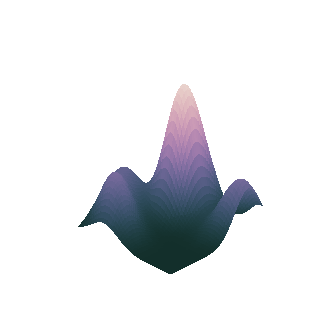
\includegraphics[width=40pt]{dist_0}};
    \node[below=-10pt of d0] (d1) {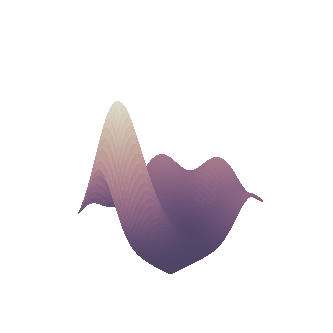
\includegraphics[width=40pt]{dist_1}};
    \node[below=-10pt of d1] (d2) {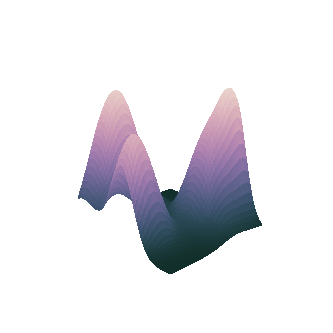
\includegraphics[width=40pt]{dist_2}};
    \node[below=-10pt of d2] (d3) {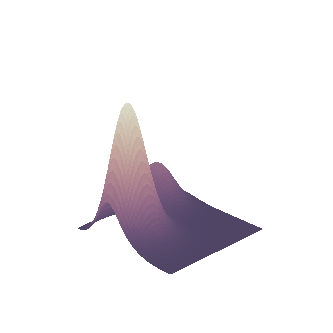
\includegraphics[width=40pt]{dist_3}};
    \node[above=-9pt of d0] (td) {\(p(\s_i)\)};

    % First columns, data
    \node[left=30pt of d0] (s0) {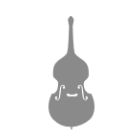
\includegraphics[width=25pt]{mixing/bass.png}};
    \node[left=30pt of d1] (s1) {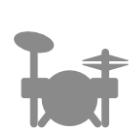
\includegraphics[width=25pt]{mixing/drums.png}};
    \node[left=30pt of d2] (s2) {
\includegraphics[width=25pt]{mixing/voice.png}};
    \node[left=30pt of d3] (s3) {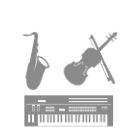
\includegraphics[width=25pt]{mixing/other.png}};
    \node[above=0pt of s0] (ts) {data};

    % Arrows frist to second
    \draw [->] (s0) to (d0);
    \draw [->] (s1) to (d1);
    \draw [->] (s2) to (d2);
    \draw [->] (s3) to (d3);
    \draw (ts) -- (td) node [above, midway,align=center] {estimate};

    % Column posterior
    \node[right=30pt of d0] (dp0) {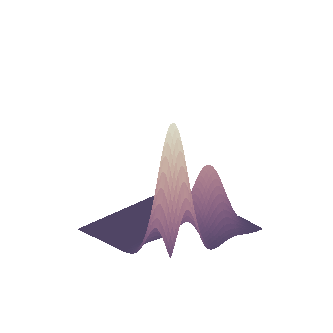
\includegraphics[width=40pt]{dist_0_post}};
    \node[right=30pt of d1] (dp1) {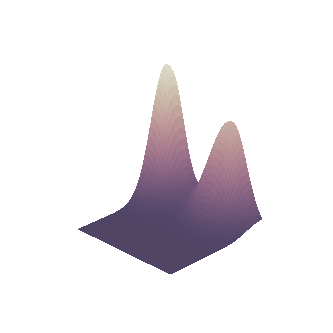
\includegraphics[width=40pt]{dist_1_post}};
    \node[right=30pt of d2] (dp2) {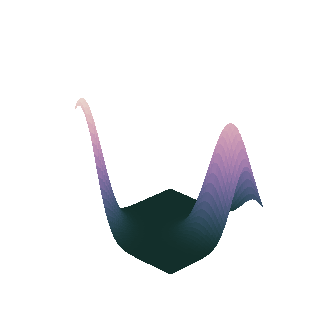
\includegraphics[width=40pt]{dist_2_post}};
    \node[right=30pt of d3] (dp3) {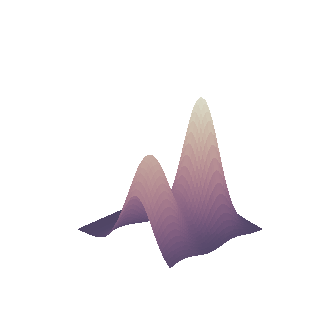
\includegraphics[width=40pt]{dist_3_post}};
    \node[above=0pt of dp0] (tp) {posterior};

    % Mix wave
    \node[above right=10pt of td] (wav) {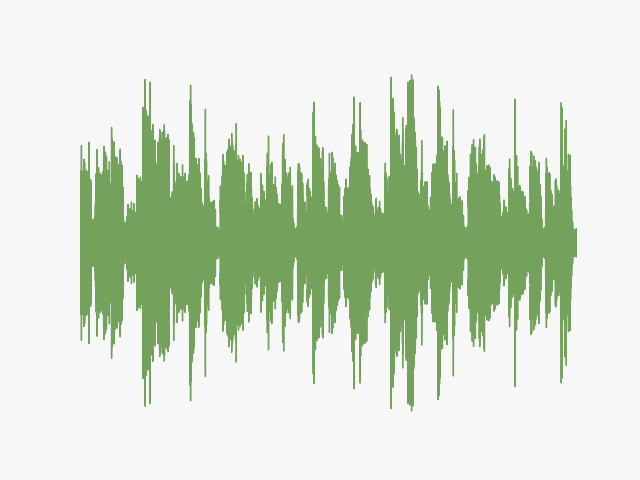
\includegraphics[width=40pt]{mixing/mix_wav.png}};
\end{tikzpicture}

    \caption{The method visualized}%
    \label{fig:method}%
    \setfloatalignment{b}%
\end{figure}

Looking back at the graphical model in \cref{fig:graphical_model}, it implies the following factorization:

\begin{align}
    p(\m)
    &= \∫^N p(\s_1,\…,\s_N,\m) \,d^N \s\\
    &= \∫^N p(\m | \s_1,\…,\s_N) \· p(\s_1,\…,\s_N) \,d^N \s\\
    &= \∫^N p(\m | \s_1,\…,\s_N) \· p(\s_1) \cdots p(\s_N) \,d^N \s
\end{align}

While the conditional \(p(\m | \s_1,\…,\s_N)\) is not even probabilistic, as the mix is generated deterministically with the mean of the sources, the model posterior \(p(\s_1,\…,\s_N | \m)\) is intractable and precisely what we are interested in. Again we want to make it clear that this setup changes the typical optimization target, as seen in other source separation approaches. We factorize the distribution \(p(\m)\) of mixed songs, only then to extract the most likely \I{latent} components that generate this mix, the sources. Therefore we are explicitly modelling the generative process of the mixed songs, and only implicitly the separation task.

Already with the graphical model we introduce a fairly big assumption, namely that we can model the source distributions independently from each other when modeling the joint:

\begin{align}
    p(\m,\s_1,\…,\s_N) &\equiv p(\m|\s_1,\…,\s_N) \· \Π_k^N p(\s_k)\label{eq:assumption}
\end{align}

Intuitively this assumption does not, in general, hold for the musical domain. We can expect a different behaviour for a \I{guitar} in a song involving a second source like a \I{percussion set}. The joint of those two models is different than their independent densities~\footnote{A practical counter-example: If learning the behaviour of drums, only from solo drum recordings, one will encounter complex rhythms and sounds. In many rock genres drums often exhibit simpler sounds, providing beat and tempo. These two distributions are not the same.}. Nevertheless, this assumption is crucial to be able to model the prior instrumental models without needing the tuples \((\s_1,\…,\s_N)\) of co-occurring stems.

The general process is as follows:

First, because we assumed in our graphical model the latent sources to be independent, there exists a probability distribution \(p(\s_k)\) for each source \(k\). Thereout we need to choose a model which gives the parametrized approximated prior \(p_{\B{\θ}}(\s_k)\) with the parameters \(\B{\θ}\) which we optimize with the samples from \(\D_k\).

Second, for each source, there exists a posterior given a mix \(p(\s_k | \m)\) from which we want to draw samples. Here two approaches are possible. Either we can propose an approximate posterior \(\aprxpost\), which is trained to minimize the divergence from the previously trained and fixed corresponding prior (VAE setting). Or, we can sample directly from the posterior using Stochastic Gradient Langevin Dynamics (SGLD)~\cite{wellingBayesian2011} without explicitly approximating the posterior distribution (sampling setting). Both optimization, either training or sampling, happen under the mixing constraint:

\begin{align}
    \Σ_{k=1}^N \s_k = \m
\end{align}

When using the VAE setting we then can sample from each posterior to retrieve a set of (approximately) correct source tracks. In the case of using Langevin dynamics, the iterative sampling will directly give this set from the prior distributions.

Thinking in the common terms of the VAE we need to choose:

\begin{enumerate}
    \item a parametrization \(p_{\B{\θ}}(\s_k)\) of the \I{prior} distribution
    \item a parametrized approximate posterior distribution \(\aprxpost\) with parameters \(\B{\η}\)
    \item a parametrized \I{encoder} which gives the parameters for the posterior distribution \(\texttt{Encoder}_{\B{\φ}}(\m) = \B{\η}\)
    \item a \I{decoder} which returns the input \(\m\) from the latents \linebreak \({\texttt{Decoder}(\{\s_1,\…,\s_N\}) = \m}\)
\end{enumerate}

As stated before the decoder in our case is the mean function, thus not probabilistic and without parameters. It is certainly possible to parametrize the decoder with trainable parameters. This would imply though that the latent samples are not in the \I{direct form} of the source sounds but under an (unknown) transformation.

\section{Modeling the priors}
The first step in the training procedure is the training of the independent source priors \(p(\s_k)\). We have to choose a model for estimating the density that results in smooth, tight densities but also is capable enough to capture the complex data space of audio data. We choose to estimate the priors, with flow models for which we gave an overview in \sref{subsec:flows}. The invertibility of the flow gives us the ability to sample from the priors, which is necessary for the sampling-based approach. For the variational-based approach sampling is not necessary, nevertheless we utilize the same generative priors for both experiments. For different representations of the input, different network architectures are more suited. We experiment both with using directly the time-domain wave but also modelling on top of a spectral transformation of the time-domain data.

The two main variants of normalizing flows we build our priors from are the RealNVP and Glow. Their most important difference is the different formulation of the coupling layers. For the coupling layers, we have to split the layer input into two equally sized subsets, one of whom will be transformed using an invertible transformation parametrized by the other. The RealNVP masks the data spatially or over the channels. When done spatially a checkerboard binary mask is used (same for all channels), for the channel variant the channels are assigned in an even-odd switching. Glow, on the other hand, learns a \(1\× 1\)-convolution which permutes the data channel-wise and than just splits the data along the channel dimension into two. For both RealNVP and Glow prior work exists specifically adapting the architecture to the time-series domain by integrating WaveNet modules, FloWaveNet~\cite{kimFloWaveNet2019} and WaveGlow~\cite{prengerWaveGlow2018}, respectively.
\itodo{Remove Glow if no experiment will use it…}

For the case of the time-domain representation, the data has only one channel (mono-audio). Therefore a Glow-like shuffling of channels is not possible and we resort to using spatial masking for the coupling layers. A one-dimensional mask is used over the time dimension. In the case of using a spectral representation of the audio data, the input samples have a lower time resolution but instead the frequency distribution over a deeper channel dimension. Therefore we can also experiment with channel-shuffling.

We make it clear that the success of this method depends strongly on the expressiveness and smoothness of the learned prior models. In the case of learning the posterior, variational learning will fit the posterior distribution under the prior distribution. If the prior does not contain enough variation of the actual data distribution, the de-mixing model cannot fit a conditional posterior similar to the sample in the mixed song. In the case of the sampling approach, this constraint is even more stressed. The mixed is generated by iteratively sampling from the set of prior distributions, any possible source sample, therefore, has to be found on the manifold of the prior. If any of the priors does not capture the full variations of the data distributions, neither method will be able to extract the correct separated sources.

More practically we again point out the high difficulty of modelling audio data. As laid out in \sref{subsec:audio} audio consists of information at greatly different resolutions. A generative model of an instrument has to model the low-range components, e.g.\ pitch, timbre, tremolo and high-range components, e.g.\ notes and rhythm.

\subsection{Prior architecture}

See the visualization of the prior model's architecture in \cref{fig:prior_network}. We construct normalizing flow models, following the description in \textcite{kimFloWaveNet2019}.

The flow network, at the highest level, consists of \(n_b\) context blocks, each of whom contain one squeeze operation and \(n_f\) flows. The squeeze operation halves the length of the signal by doubling the number of channels. By doing so, we effectively double the receptive field of the WaveNet operators in the affine couplings. One flow contains one affine coupling layer after which the masking for the coupling (\I{even}/\I{odd}) is inverted. Before the coupling layer, we apply activation normalization~\cite{kingmaGlow2018}. The affine coupling is applying an affine transformation on the \I{odd} set of the input, with scale \(\s\) and translation \(\B{t}\) coming from the \I{even} input put through a \I{non-causal} WaveNet.

\begin{figure}[t]
    
\begin{tikzpicture}[every node/.style={scale=0.8}]
    \tikzstyle{box}=[rectangle,draw,minimum width=25mm,minimum height=5.55mm,fill=black!10]
    \tikzstyle{hbox}=[box,minimum width=12mm,fill=yellow!10]
    \tikzstyle{label}=[rotate=-90,yshift=5]

    \begin{scope}
        \node (z) {\(z\)};
        \coordinate[below=10pt of z] (belowz) {};
        \coordinate[below=10pt of belowz] (aboveflow) {};
        \node[below=7pt of aboveflow,box,fill=orange!40] (flow)    {Flow};
        \coordinate[below=7pt of flow] (belowflow) {};
        \node[below=13pt of belowflow,box,fill=green!40] (squeeze) {Squeeze};
        \coordinate[below=10pt of squeeze] (abovex) {};
        \node[below=10pt of abovex] (x) {\(x\)};


        \draw[->] (x) to (abovex) to (squeeze);
        \draw[->] (squeeze) to (flow);
        \draw[->] (flow) to (belowz) to (z);

        \draw (belowz) -| (1.7, -2) node[label] {\(\times n_f\)} [->]|- (abovex);
        \draw (aboveflow) -| (1.1,-1.35) node[label] {\(\times n_b\)} [->]|- (belowflow);

        \begin{pgfonlayer}{background}
            \filldraw [inner sep=50pt,line width=4mm,black!10]
              (-1.15,-0.9) rectangle (1.15,-3);
        \end{pgfonlayer}
    \end{scope}

    \begin{scope}[xshift=4cm]
        \node (end) {};
        \node[box,below=23pt of end] (corder) {change order};
        \node[box,below=10pt of corder,fill=aqua!40] (ac) {Affine coupling};
        \node[box,below=10pt of ac] (an) {ActNorm};
        \node[below=12pt of an] (start) {\(z\)};

        \draw[->] (start) to (an);
        \draw[->] (an) to (ac);
        \draw[->] (ac) to (corder);
        \draw[->] (corder) to (end);

        \begin{pgfonlayer}{background}
            \filldraw [inner sep=50pt,line width=4mm,orange!20]
              (-1.15,-0.9) rectangle (1.15,-3);
        \end{pgfonlayer}
    \end{scope}

    \begin{scope}[xshift=8cm]
        \coordinate[yshift=-10pt] (end) {};
        \node[hbox,left=1pt of end] (oodd) {\({out}_{odd}\)};
        \node[hbox,right=1pt of end] (oeven) {\({out}_{even}\)};

        \node[hbox, below=50pt of oodd] (wn) {WN};
        \node[hbox, below=15pt of oeven] (trans) {\(\exp{s} \· x + t\)};

        \node[hbox,below=80pt of oodd] (iodd) {\({in}_{odd}\)};
        \node[hbox,below=80pt of oeven] (ieven) {\({in}_{even}\)};

        \draw[->] (iodd) to (wn);
        \draw[->] (trans) to (oeven);
        \draw[->] (ieven) to node[label] {\(x\)} (trans);
        \draw[->] (wn) |- node[label,xshift=20pt] {\(s, t\)} (trans);
        \draw (iodd.west) -| (-1.45, -1.3) [->]|- (oodd);

        \begin{pgfonlayer}{background}
            \filldraw [inner sep=50pt,line width=4mm,aqua!20]
              (-1.15,-0.9) rectangle (1.25,-3);
        \end{pgfonlayer}
    \end{scope}
\end{tikzpicture}

    \caption{The building blocks for the prior model. The model consists of \(n_b\) blocks (left). Each block consists of \(n_f\) flows (middle). In each flow we apply activation normalization, followed by the affine coupling (right), after which the binary mask for the even/odd mapping is inverted. The affine coupling layer uses a WaveNet with the \I{even} set as the input to output scaling \(\log s\) and translation \(t\) which which the \I{odd} set is transformed.}%
    \label{fig:prior_network}
\end{figure}

\begin{figure}
    \hspace*{-25pt}\begin{tikzpicture}
    \node                   (s0) {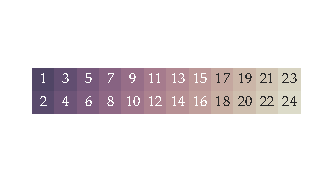
\includegraphics[width=1.2in]{squeeze_0}};
    \node[right=50pt of s0] (s1) {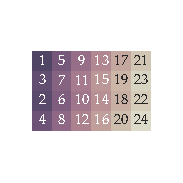
\includegraphics[width=0.9in]{squeeze_1}};
    \node[right=50pt of s1] (s2) {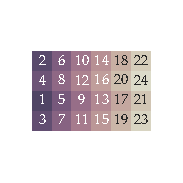
\includegraphics[width=0.9in]{squeeze_2}};

    \graph {(s0) ->["squeeze"] (s1) ->["flip"] (s2)};
\end{tikzpicture}
%
    \caption{Flip and squeeze operation for the coupling layers. The squeeze operation doubles the channels and halves the length while the flip operation inverts the tensor along the channel dimension.}%
    \label{fig:squeeze}%
\end{figure}

The \I{even}/\I{odd} masking for the coupling layer is simply achieved by splitting the channel dimension into two equal parts. Flipping the masking exchanges the top half of channels with the bottom half. No channel transformation of the channels is learned as in Glow. Further observe that through the repeated squeeze operation the masking implicitly includes a checkerboard pattern on the temporal dimension, similar to the explicit pattern used in RealNVP\@.

As explained in \cref{subsec:flows} the invertible flow \(f(\·)\) network directly maps the data space into a prior distribution \(p(\z)\). Through the invertibility we can directly optimize the log probability with the change of variable formula:

\begin{equation}
    \log p(\x) = \log p(f(\x)) + \log\det\left(\pf{f(\x)}{\x}\right)%
    \label{eq:priorflow_likelihood}
\end{equation}

Our network consists of \(n_b\) blocks with each \(n_f\) flows each with one activation normalization layer \(f_{\t{AN}}\) and an affine coupling layer \(f_{\t{AC}}\). Therefore the log-determinant becomes:

\begin{equation}
    \log\det\left(\pf{f(\x)}{\x}\right)
    = \Σ_i^{n_b \· n_f} \log\det\pf{f_{\t{AN}}(\x)}{\x} + \log\det\pf{f_{\t{AC}}(\x)}{\x}
\end{equation}

The activation normalization layer \(f_{\t{AN}}\) learns an affine transformation per channel \(i\):

\marginnote[2.5em]{The inverse is:\\\(f^{-1}_{\t{AN}}(\B{y}_i) = \÷{\B{y}_i -  t_i}{s_i}\)}
\begin{equation}
    f_{\t{AN}}^i(\x_i) = s_i \· \x_i + t_i
\end{equation}

The log-determinant is easily computed with\footnotemark[\value{footnote}]:

\begin{equation}
    \log\det\pf{f_{\t{AN}}(\x)}{\x}
    = T \· \Σ_i^C \log |s_i|%
    \label{eq:priorflow_det1}
\end{equation}

where C is the number of channels and T is the length of the signal.

For the affine coupling layer, the log-determinant is made tractable by only transforming half the elements in each application. The coupling transforms the \I{odd} part as follows:

\begin{align}
    \log\B{s}, \B{t} &= \t{WN}({in}_{odd})\\
    {out}_{odd} &= f_{\t{AC}}({in}_{odd}) = \÷{{in}_{odd} - \B{t}}{\B{s}}
\end{align}
\marginnote[-4em]{The inverse is:\\\(f^{-1}_{\t{AC}}({out}_{odd}) = {out}_{odd}\·\B{s} + \B{t}\)}

where \(\t{WN}(\·)\) is a WaveNet. The Jacobian of the coupling function is a lower triangular matrix\cite{dinhDensity2017} because of which the log-determinant becomes the product of the diagonal elements:

\begin{equation}
    \log\det\pf{f_{\t{AC}}(\x)}{\x}
    = - \Σ \B{s}%
    \label{eq:priorflow_det2}
\end{equation}

The purpose of the invertible flow is it to project the complex data distribution into a tractable defined prior distribution. In most cases, as in this, the prior \(p(\z)\) is set to be a factorized Gaussian distribution with zero mean and variance of one. As such the likelihood of \(f(\x) \sim p(\z)\) can be evaluated with:

\begin{equation}
    \log p(f(\x)) = -\÷{1}{2}(\log(2\· \π)) + {f(\x)}^2%
    \label{eq:priorflow_ll}
\end{equation}

To train the model we maximize the likelihood in \cref{eq:priorflow_likelihood} which we is the sum of the parts in \cref{eq:priorflow_det1,eq:priorflow_det2,eq:priorflow_ll}. Optimization is done in mini-batches with the Adam optimzer~\cite{kingmaAdam2017} and a decaying learning rate scheme.

It is noted that the likelihood under the prior is computed ``pixel''-wise\footnote{time-points in our sound case}. While for the optimization the actual loss on which the optimizers performs update steps is the mean likelihood, we can use the trained prior flow to assign a likelihood map to an input signal where each log-likelihood value is depending on this values receptive field.

\subsection{WaveNet}
In the affine coupling layer we utilize a \I{non-causal} WaveNet for generating the scale \(\log \s\) and translation \(\B{t}\) values. The WaveNet is non-causal because the filters are centred, as such the receptive field of an output value is symmetrically in the past and future input space. The kernel size is fixed to 3. The WaveNet is using the original gated convolution scheme described in \sref{ch:background}. Appended to the last skip connection output are two additional one-dimensional convolutional layers, each preceded by a ReLU\@. The last convolutional layer is initialized to zero. By that we initialize the affine transformation of the coupling layer to the identity at the beginning of training, helping to stabilize optimization. The last layer outputs both scaling and translation factors. Learning those factors with weight sharing does not change the formulation of the coupling layer, as the log-determinant does not depend on the network. Learning them in the same network might increase efficiency, as well as, increasing implementation simplicity. The WaveNet completely consists of convolutional operations. As such it can be applied to one-dimensional signals of variable length.

\section{Sampling from the posteriors}
After having estimated the \(N\) prior distributions the first possibility for retrieving sample estimates \(\s_k\) is sampling from the posterior using Langevin dynamics~\cite{wellingBayesian2011}. With Stochastic Gradient Langevin Dynamics (SGLD) we can sample from \(\s_i \sim p(\· | \m)\) without computing, explicitly, the posterior \(p(\s_i | \m)\). For a overview of SGLD see~\sref{sec:langevin}.

Starting with the update step in SGLD we reformulate the update with our problem constraint:

\begin{align}
    \s_k^{(t+1)}
    &= \s_k^{(t+1)} + \η \· \∇_{\s_k}\log{p(\s_k^{(t)}|\m)} + 2\sqrt{\η}\ε_t\\
    &= \s_k^{(t+1)} + \η \· \∇_{\s_k}\left[\log{p(\m|\s_k)} + \log{p(\s_k)} - \log{p(\m)}\right] + 2\sqrt{\η}\ε_t\\
    &= \s_k^{(t+1)} + \η \· \∇_{\s_k}\left[\log{p(\m|\s_k)} + \log{p(\s_k)} \right] + 2\sqrt{\η}\ε_t\\
    &= \s_k^{(t+1)} + \η \· \left[\|\m - \÷{1}{N}\Σ_{j}^N \s_j^{(t)}\| + \∇_{\s_k}\log{p(\s_k)}\right] + 2\sqrt{\η}\ε_t
\end{align}\marginnote[-1.2in]{\(\log{p(\m)}\) is independent from \(\s_k\) therefore no gradient.}

\(\η\) is the update step size and \(\ε_t \sim \N(0,\1)\).

Note that the final formulation of the update step is simply a constrained greedy hill-climb under the prior model with added Gaussian noise. Intuitively the artificially noised update makes it harder for the greedy optimization to get stuck in local minima of the prior surface.

\begin{algorithm}
    \begin{algorithmic}[1]
        \For{\(t=1\…T\)}
            \For{\(k=1\…N\)}
                \State\(\ε_t \sim\N(0, \1)\)
                \State\(\Δ\s_k^t \gets\s^t + \η \· \∇\log{p(\s^t)} + 2\sqrt{\η}\ε_t\)
            \EndFor%
            \For{\(k=1\…N\)}
                \State\(\s_k^{t+1} \gets\Δ\s_k^t -\÷{\η}{\σ^2}\· [\m  - \÷{1}{N}\Σ^N_i \s_i^t]\)
            \EndFor%
        \EndFor%
    \end{algorithmic}
    \caption{The Langevin sampling procedure for source separation is fairly straight forward. For a fixed number of steps \(T\) we sample we take a step into the direction of the gradient under the priors and the gradient of the mixing constraint while adding Gaussian noise \(\ε_t\).}%
    \label{alg:langevin_sampling}%
    \setfloatalignment{t}
\end{algorithm}

The idea of using SGLD in combination with deep parametrized priors was, concurrently to this work, introduced in \textcite{jayaramSource2020}. The authors empirically show that
\[\E\left[{\|\∇_{\s}\log{p_{\σ}(\s)}\|}^2\right] \propto \nf{1}{\σ^2}\]
They argue that this surprising proportionality is stemming from the severe non-smoothness of the prior model. If the prior model, in the extreme case, exhibits a Dirac delta peak as the probability mass, then the estimation of the gradient with added Gaussian noise will it-self be proportional to the Gaussian. From there the authors argue, that the prior models have to be trained with noised samples, where the added noised is proportional to later used estimator noise.

\section{Modeling the posteriors}
Instead of formulating a sampling regime for approaching \(\s_k\) we can also use the prior models to variationally train a model to estimate the parameters of an approximate posterior \(\aprxpost\). While estimating the true posterior \(p(\s_k|\m)\) is intractable, we choose a certain parametrized distribution as an approximation of the posterior and optimize the parameters to align with the true one.

We follow the same steps as previously shown generally for the latent variable models. First, we introduce an approximate posterior \(\aprxpost\) for each source channel. Next, we express the mix density as the expectation over those posteriors:

\begin{align}
    \log p(\m)
    &= \E_\aprxpost^N \left[ \log p(\m) \right]\label{eq:expectation_over_approx_post}
\end{align}

From here we introduce the approximate posteriors in the expectation as before, just now for \(N\) separate priors:

\begin{fullwidth}
    \newcommand{\post}{ p (\s_1,\…,\s_N|\m) }
    \begin{align}
        \E_\aprxpost^N \left[ \log p(\m) \right]
        &= \E_\aprxpost^N \left[ \log \÷{p(\m,\s_1,\…,\s_N)}{\post} \right]\\
        &= \E_\aprxpost^N \left[ \log \÷{p(\m|\s_1,\…,\s_N) \· \Π_k^N p(\s_k)}{\Π_k^N \aprxpost} + \log \÷{\Π_k^N \aprxpost}{\post} \right]
    \end{align}

\end{fullwidth}

Note that again we use the assumption in~\cref{eq:assumption} to factorize the joint. This assumption is not being used for the independent approximate posteriors. While the true posterior certainly is the posterior of the joint source model, we choose our approximate posteriors to be independent. The expectation in~\eqref{eq:expectation_over_approx_post} over those is still correct. The error arising from the independence assumption is captured in the thightness of the ELBO\@.

We arrive at the ELBO by leaving out the divergence of the approximate posterior to the true posterior:

\begin{fullwidth}
    \begin{align}
        \E_\aprxpost^N \left[ \log p(\m) \right]
        &\geq \Σ_k^N \E_\aprxpost \left[ \log \÷{p(\s_k)}{\aprxpost} \right]
             +\E_\aprxpost \left[ p(\m|\s_1,\…,\s_N) \right]
    \end{align}
\end{fullwidth}

The lower bound, as in the normal VAE, will be our optimization target for training the inference models that give the variational parameters \(\B\φ_k\). We can also formulate the objective for just one source, as the Encoders are trained independently\footnote{While the optimization of the Encoders is independent, the training is, of course, concurrent as the mixing condition depends on all \(N\) source samples.}. Thus we come to:

\begin{fullwidth}
    \begin{align}
        \E_\aprxpost \left[ \log p(\m) \right]
        &\geq \E_\aprxpost \left[ \log \÷{p(\s_k)}{\aprxpost} \right]
        +\E_\aprxpost \left[ p(\m|\s_1,\…,\s_N) \right]\\
        &=    \E_\aprxpost \left[ \log \÷{p(\s_k)}{\aprxpost} \right]
        +{\|\m - \÷{1}{N}\Σ_j^N \s_j\|}\label{eq:final_elbo}
    \end{align}
\end{fullwidth}

The Kullback-Leibler divergence term is computationally expensive, therefore the divergence is the stochastic estimate using just one mini-batch.

As both the prior \(p(\s_k)\) and the approximate posterior \(\aprxpost\) are parametrized by deep neural network, the gradient of \cref{eq:final_elbo} is tractable with respect to the mini-batch.

With the optimization regime set up, we have to choose a fitting posterior distribution and the deep neural network which computes its parameters from data. In many typical VAE settings, the prior density is a fixed probability distribution, typically a multivariate normal distribution and accordingly the approximate posterior also is set to be a normal distribution. As our prior is a greatly complex distribution estimated by the flow, we are not incentivized by this to choose the posterior accordingly. Further, we have the benefit of knowing our posteriors to model sound in the time-domain. Therefore we take a look at the distributions induced by our data samples, in the two cases of the Toy Data and the real musical recordings. For a more in-depth discussion of the datasets see \sref{ch:experiments}.
\begin{marginfigure}[-20em]
    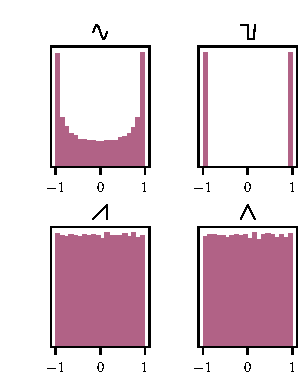
\includegraphics{toy_dist}
    \caption{The logits of different classes of the different outputs}%
    \label{fig:toy_dist}
\end{marginfigure}%
In the case of the \B{Toy data}, the waveforms are regular, simple patterns. If we plot the histograms of an example wave for each source class (\cref{fig:toy_dist}), the probability distribution induced by those sources is again simply formulated. Both the \I{triangle} and \I{sawtooth} waves induce a uniform distribution, the \I{square} wave collapses on the only two values contained in the signal (the maxima) and the sine wave also gives a symmetrical distribution with the values around the maxima greatly more likely. We propose modelling these posteriors with a \B{Beta distribution}.
\begin{marginfigure}
    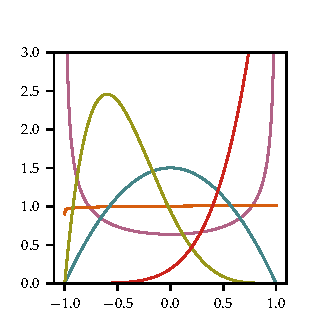
\includegraphics{beta}%
    \caption{Beta distributions with different concentrations \(\α\) and \(\β\)}%
    \label{fig:beta}
\end{marginfigure}

To learn the variational parameters \(\B{\φ}\) of the encoder network \(\texttt{Encoder}_{\B{\φ}}(\m) = \B{\η}\) which infers the parameters \(\B{\η}\) of the approximate posterior we need the gradient of samples taken from the posterior with respect to the parameters. The Beta distribution is parametrized by the two concentrations \(\α\) and \(\β\). Therefore we need:

\begin{equation}
    \pf{}{\B{\α}} \B{z}\ ,\quad\pf{}{\B{\β}} \B{z} \quad \B{z} \sim \aprxpost
\end{equation}

As described in \sref{sec:dlvm} with choosing a Gaussian posterior, one can use the reparametrization trick to get low-variance gradients, simply and efficiently. In the case of using a Beta posterior, the reparametrization trick is not applicable. There exists multiple approaches to compute implicit gradients through approximate differentiation of different probability distribution. \textcite{figurnovImplicit2019} provides an new fast general gradient estimator. You employ this estimator in the form that it is implemented in the PyTorch framework.

\begin{algorithm}
    \begin{algorithmic}[1]
        \For{\(x\∈\D_k\)}
        \EndFor%
    \end{algorithmic}
    \caption{Training of the approximate posterior.}%
    \label{alg:posterior_training}%
\end{algorithm}

\section{Difficulties of this method}
\begin{enumerate}
    \item Good prior densities
\end{enumerate}
